\documentclass{article}
\usepackage{pgfplots}
\pgfplotsset{compat=1.18}

\begin{document}

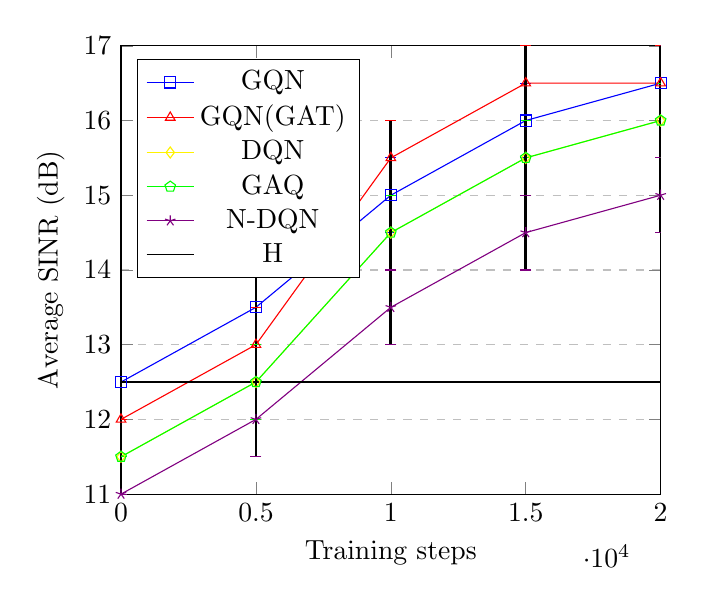
\begin{tikzpicture}
    \begin{axis}[
        xlabel={Training steps},
        ylabel={Average SINR (dB)},
        xmin=0, xmax=20000,
        ymin=11, ymax=17,
        xtick={0,5000,10000,15000,20000},
        ytick={11,12,13,14,15,16,17},
        legend pos=north west,
        ymajorgrids=true,
        grid style=dashed,
    ]
    
    \addplot[
        color=blue,
        mark=square,
        error bars/.cd,
        y dir=both,
        y explicit,
        error bar style={line width=1pt, draw=black},
    ]
    coordinates {
        (0,12.5) +-(0,0)
        (5000,13.5) +-(0,0.5)
        (10000,15.0) +-(0,0.5)
        (15000,16.0) +-(0,0.5)
        (20000,16.5) +-(0,0.5)
    };
    \addlegendentry{GQN}
    
    \addplot[
        color=red,
        mark=triangle,
        error bars/.cd,
        y dir=both,
        y explicit,
        error bar style={line width=1pt, draw=black},
    ]
    coordinates {
        (0,12.0) +-(0,0)
        (5000,13.0) +-(0,0.5)
        (10000,15.5) +-(0,0.5)
        (15000,16.5) +-(0,0.5)
        (20000,16.5) +-(0,0.5)
    };
    \addlegendentry{GQN(GAT)}
    
    \addplot[
        color=yellow,
        mark=diamond,
        error bars/.cd,
        y dir=both,
        y explicit,
        error bar style={line width=1pt, draw=black},
    ]
    coordinates {
        (0,11.5) +-(0,0)
        (5000,12.5) +-(0,0.5)
        (10000,14.5) +-(0,0.5)
        (15000,15.5) +-(0,0.5)
        (20000,16.0) +-(0,0.5)
    };
    \addlegendentry{DQN}
    
    \addplot[
        color=green,
        mark=pentagon,
        error bars/.cd,
        y dir=both,
        y explicit,
        error bar style={line width=1pt, draw=black},
    ]
    coordinates {
        (0,11.5) +-(0,0)
        (5000,12.5) +-(0,0.5)
        (10000,14.5) +-(0,0.5)
        (15000,15.5) +-(0,0.5)
        (20000,16.0) +-(0,0.5)
    };
    \addlegendentry{GAQ}
    
    \addplot[
        color=violet,
        mark=star,
        error bars/.cd,
        y dir=both,
        y explicit,
        error bar style={line width=1pt, draw=black},
    ]
    coordinates {
        (0,11.0) +-(0,0)
        (5000,12.0) +-(0,0.5)
        (10000,13.5) +-(0,0.5)
        (15000,14.5) +-(0,0.5)
        (20000,15.0) +-(0,0.5)
    };
    \addlegendentry{N-DQN}
    
    \addplot[
        color=black,
        mark=none,
        error bars/.cd,
        y dir=both,
        y explicit,
        error bar style={line width=1pt, draw=black},
    ]
    coordinates {
        (0,12.5) +-(0,0)
        (5000,12.5) +-(0,0)
        (10000,12.5) +-(0,0)
        (15000,12.5) +-(0,0)
        (20000,12.5) +-(0,0)
    };
    \addlegendentry{H}
    
    \end{axis}
\end{tikzpicture}

\end{document}